\documentclass[a4paper,12pt]{article}

\usepackage[14pt]{extsizes}
\usepackage{cmap}					% поиск в PDF
\usepackage{mathtext} 				% русские буквы в формулах
\usepackage[T2A]{fontenc}			% кодировка
\usepackage[utf8]{inputenc}			% кодировка исходного текста
\usepackage[english,russian]{babel}	% локализация и переносы
\usepackage{graphicx}
\usepackage{geometry}
\usepackage{amsmath}
\usepackage{amssymb}
\usepackage[table]{xcolor}
\setlength\extrarowheight{2pt}
\usepackage{multirow}


\geometry{verbose, a4paper, tmargin=2cm, bmargin=2cm, lmargin=3cm, rmargin=2cm}
\author{Vysotsky Maxim}
\title{Отчёт}
\date{2024}

\begin{document}
	\begin{titlepage}
		\begin{center}
			{Министерство науки и высшего образования Российской Федерации
				НОВОСИБИРСКИЙ НАЦИОНАЛЬНЫЙ ИССЛЕДОВАТЕЛЬСКИЙ
				ГОСУДАРСТВЕННЫЙ УНИВЕРСИТЕТ (НГУ)}
		\end{center}
		\begin{center}
			{Физический факультет}
		\end{center}
		\begin{center}
			{Кафедра общей физики}
		\end{center}
		
		
		\vspace{7cm}
		{
			\begin{center}
				{\bf Лабораторная работа №4.1}\\
				Компенсационные методы измерений
			\end{center}
		}
		\vspace{2cm}
		\begin{flushright}
			{Руководитель:\\ Старший преподаватель\\
				Яцких А. А.\\
				Работу выполнил:\\
				Высоцкий М. Ю.\\
				\vspace{0.2cm}
				гр. 24301}
		\end{flushright}
		\vspace{3cm}
		\begin{center}
			Новосибирск, 2024
		\end{center}
	\end{titlepage}


\section{Теоретическое введение}
\textbf{Цель работы:} изучение компенсационных методов измерения ЭДС, напряжений и сопротивлений. \\

\textbf{Оборудование:} 
\begin{enumerate}
    \item Потенциометр постоянного тока P4833; нормальный элемент Вестона МЭ4700; батарея питания потенциометра; нуль-индикатор, милливольтметр; термопара ТЭДС ХК (ТХК); нуль-термостат; печь с тиглем; источник питания печи (24В); регистратор ЭДС термопары.
\end{enumerate}

\begin{figure}[ht!]
    \centering
    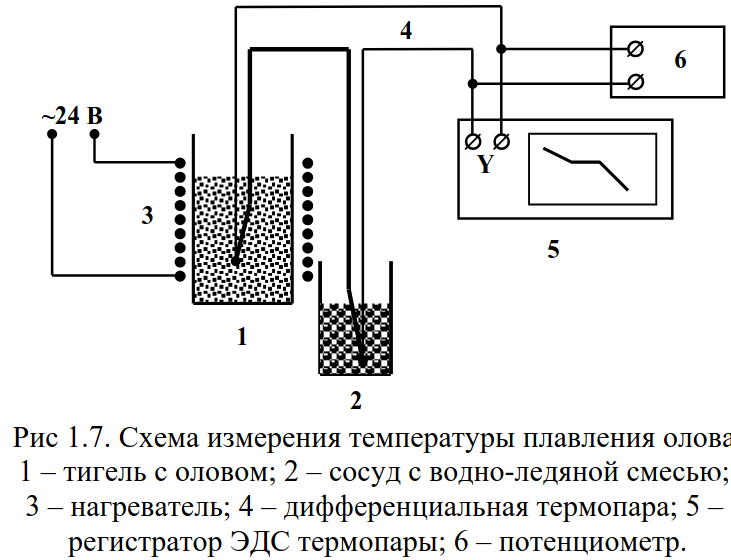
\includegraphics[scale=0.7]{scheme_1.png}
    \caption{Схема установки}
\end{figure}

\newpage
\section{Ход работы}
\subsection{Задания 1-2}
Цель задания:  измерить ЭДС термопары и определить зависимость ЭДС от температуры среды, в
которую помещён спай термопары, используя компенсационный метод измерения.

Путём помещения одного спая дифференциальной термопары в ёмкость с оловом, переходящим при нагревании в жидкое состояние и обратно при остывании, а другого в сосуд Дьюра, была измерена ЭДС термопары.

\begin{figure}[ht!]
    \centering
    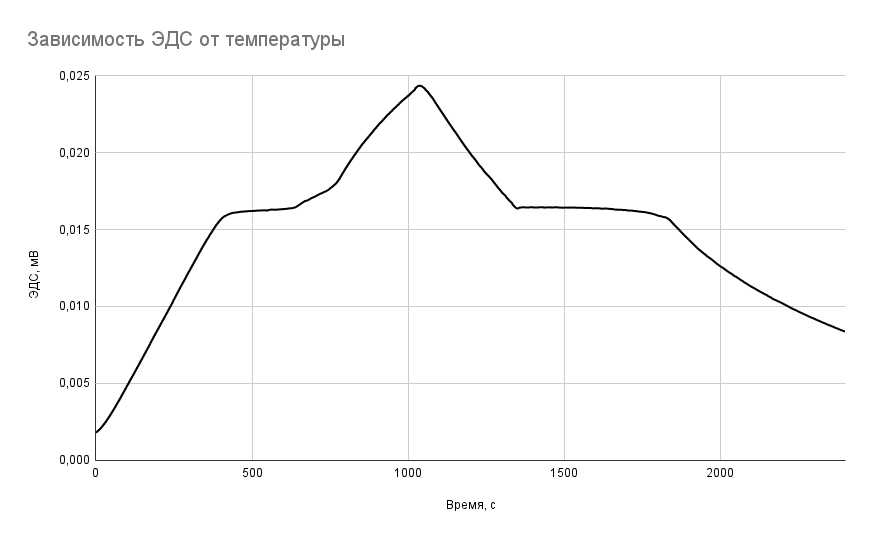
\includegraphics[scale=0.5]{eds.png}
    \caption{График зависимости $\mathcal{E}(t)$}
\end{figure}

\begin{table}[!ht]
    \centering
    \begin{tabular}{|l|l|l|l|l|}
    \hline
        Среда           & $\mathcal{E}$, мВ & $Т_{теор}$, $^{\circ} C$\\ \hline
        Комната         & 1,56   & 24\\ \hline
        Олово           & 16     & 231,9 \\ \hline
        Палец Егора     & 2,08   & 36,6 \\ \hline
        Локоть Егора    & 2,1    & 36,6 \\ \hline
        Кипящая вода    & 6,6    & 100 \\ \hline
    \end{tabular}
    \caption{Значения ЭДС и температур}
\end{table}

Далее по формуле мы ищем температуры и чувствительность термопары для разных случаев:
\begin{equation}
    t = K^-1 * \mathcal{E}
\end{equation}
\begin{equation}
    K = \frac{\mathcal{E}}{t}
\end{equation}

\begin{table}[!ht]
    \centering
    \begin{tabular}{|l|l|}
    \hline
        $К_1$       & 0,069  \\ \hline
        $t_в$       & 95,66  $^{\circ} C$\\ \hline
        $t_{пал}$   & 30,15  $^{\circ} C$\\ \hline
        $t_{лок}$   & 30,44  $^{\circ} C$\\ \hline
        $K_2$       & 0,066  \\ \hline
        $t_о$       & 242,42 $^{\circ} C$\\ \hline
        $t_{пал}$   & 31,52  $^{\circ} C$\\ \hline
        $t_{лок}$   & 31,82  $^{\circ} C$\\ \hline
    \end{tabular}
    \caption{Значения температур и чувствительности термопары}
\end{table}

\end{document}